\section{A Tree-Expanding Search with Recursive Backtracking}
\label{sec:tree_expanding_search}

In this section, we propose algorithms to solve the submodular orienteering problem on a multi-partite graph.
We use backtracking to estimate the maximum total reward and import an expanding tree to track the search process in an anytime algorithm framework. 

%The path planning problem on a multi-partite graph is equivalent with a search process on a multi-partite graph.
Each solution on the robot path is a sequence of vertices on the multi-partite graph.
We have $ X = ( x_{1}, x_{2} , \cdots , x_{T} ) = ( v_{1}, v_{2} , \cdots , v_{T} ) $.
In a manner of searching the optimal path, we can use the estimated future reward as the heuristic.
%Thus the future reward estimation becomes finding heuristic in a search problem.

Given a start node, any search problem on a graph implicitly derives an expanding tree, the root of which is the start node.
We can always map a multi-partite graph of $ T $ levels to an expanding tree that has fixed depth of $ T $. 

\begin{mydef}[\textbf{Expanding Tree}]
\label{def:expanding_tree}
An expanding tree $ G_{T} = (N, L, T) $ is a tree structure, obtained from a multi-partite graph $ G = (V, E, T) $ so that each node in the expanding tree has only one parent node.
\begin{itemize}
\item $ T $ is the depth of the tree, which is determined by the number of partitions in a multi-partite graph $ G $.
\item $ N $ is the node set. Each $ n_{t}^{i(j)} \in N $ indicates the relevant vertex in the multi-partite graph $ G $, in which $ t $ shows the index of the time partition, $ i $ shows the index of the corresponding vertex from within that partition and $ (j) $ shows the index of a vertex in $ V(t-1) $ that has an out edge to vertex $ i $.
\item $ L $ is the directed link set. $ (n^{i(k)}_{t}, n^{j(i)}_{t+1})  \in L $ is determined by $ (v^{i}_{t}, v^{j}_{t+1} ) \in E $.

\end{itemize}
\end{mydef}

Figure \ref{fig:multipartite_expandingtree} shows an example of how a vertex in a multi-partite graph is mapped to nodes in a corresponding expanding tree. The red edges form both a path on the multi-partite graph and a path on the expanding tree in order to show that paths are preserved in the mapping. 

We can see that each vertex $ v^{i}_{t} $ in the multi-partite graph can map to several nodes $ n^{j(i)}_{t+1} $ in the expanding tree, the number of which is $ deg^{+}(v^{i}_{t})$. Each node $ n^{j(i)}_{t+1} $ in the tree maps to only one vertex, which is denoted as $ v(n^{j(i)}_{t+1}) $.

Each path in an expanding tree is derived from a unique path in a corresponding mutli-partite graph.
For a node $ n_{t}^{i(j)} $, we use $ path(n_{t}^{i(j)}) $ to denote the implicit path from start position to corresponding vertex in the multi-partite graph.
The cardinality of $ path(n_{t}) $ is $ t $.
We have property \ref{prop:path}.
For simplicity of notation, we will use $ n_{t} $ instead of $ n_{t}^{i(j)} $ and $ v_{t} $ instead of $ v_{t}^{i} $ in the following sections. 

\begin{mydef}[\textbf{Complete Path}]
\label{def:complete_path}
A complete path in a path-planning problem with a planning length $ T $, is any path such that
$ | path() | = T  $ .
\end{mydef}

\begin{mydef}[\textbf{Terminal Node}]
\label{def:terminal_node}
A terminal node, defined by $ n_{T} $, is any node at level $ T $ in an expanding tree $ G_{T} = (N, L, T) $ . 
For any node $ n_{T} $, $ path(n_{T}) $ is a complete path by definition.
\end{mydef}

\begin{figure}
\centering
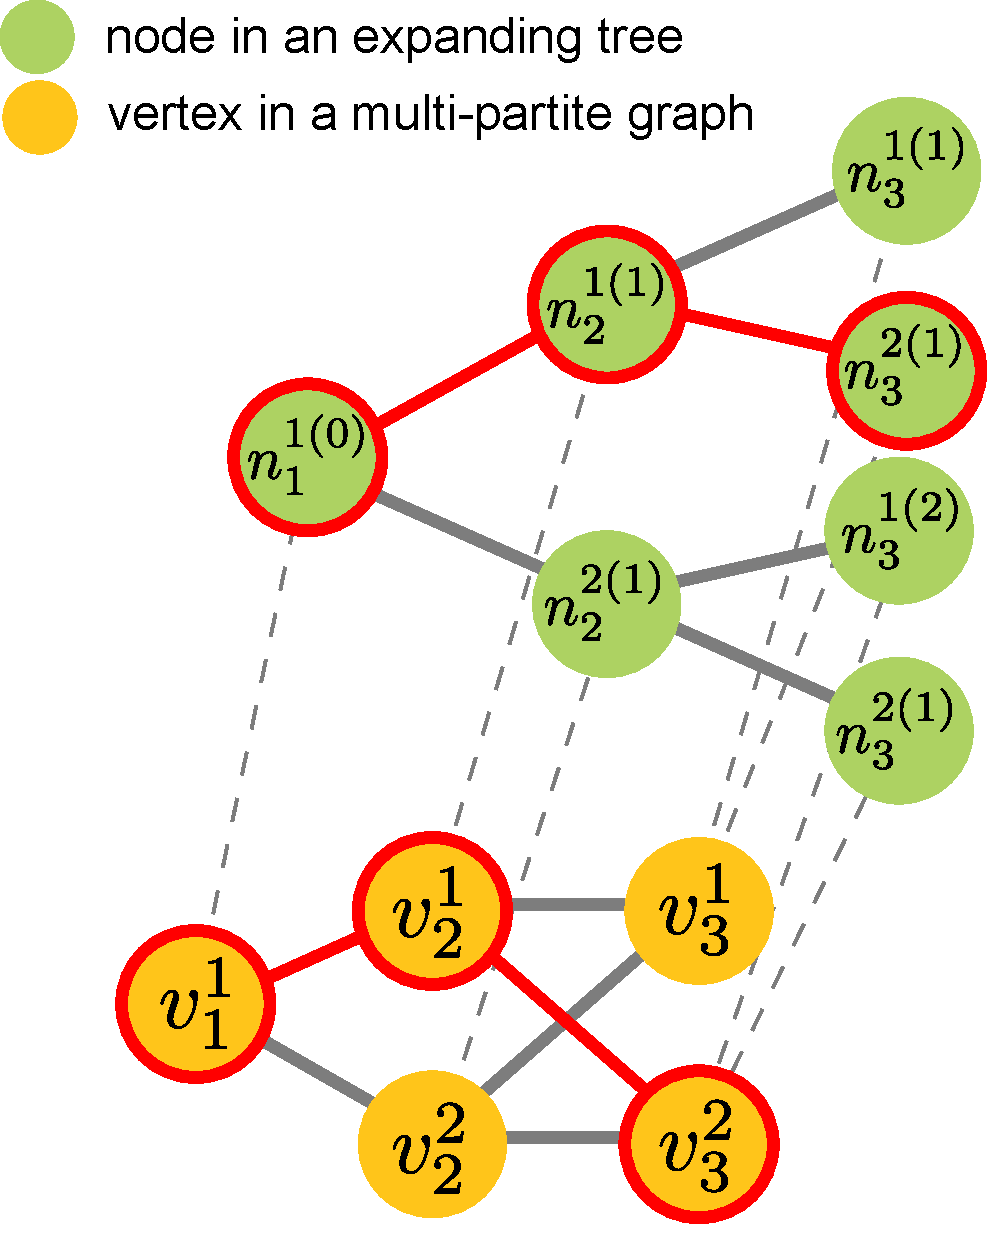
\includegraphics[width=0.4\linewidth]{./images/multipartite_expandingtree.pdf}
\caption{Mapping from a multi-partite graph to an expanding tree.}
\label{fig:multipartite_expandingtree}
\end{figure}

From the mapping between a multi-partite graph and an expanding tree, we can have Property \ref{prop:path}.

\begin{propty}
\label{prop:path}
Each node $ n_{t}^{i(j)} $, which maps to $ v_{t}^{i} $ in a multi-partite graph, implies one and only path from root to node $ n_{t}^{i(j)} $.
We define $ path(n_{t}) = ( n_{1}, n_{2} , \cdots , n_{t} ) $.
Equivalently, $ path(n_{t}) = ( v_{1}, v_{2} , \cdots , v_{t} ) $.
\end{propty}

By Property \ref{prop:orderIndependence}, we can ignore the sequence and denote $ path(n_{t}) = \{ n_{1}, n_{2} , \cdots , n_{t} \} $ as a set.

As shown in Figure \ref{fig:backtracking}, we utilize the structure of a multi-partite graph to back propagate information in estimating future reward. 
The process is given in Algorithm \ref{alg:Backtrack}.

\subsection{Backtracking Algorithm}
\label{subsec:backtrack_algorithm}

For short, we let $ f(x_{t} \mid x_{t'}=v_{t'}, x_{t'-1} = v_{t'-1} , \cdots  , x_{1} = v_{1} ) = f(x_{t} \mid v_{1}, \cdots , v_{t'}) = f(x_{t} \mid path(n_{t'})) $. 

\begin{lem}
\label{lem:submod}
When $ t' < t $, 
\begin{equation}
\label{eq:lem_submod}
f(x_{t} \mid v_{1} , \cdots , v_{t'} ) \geq f(x_{t} \mid v_{1} , \cdots , v_{t'} , \hat{x}_{t'+1} , \cdots , \hat{x}_{t-1}  ). 
\end{equation}
$ \hat{x}_{t-1} , \cdots , \hat{x}_{t'+1} $ indicate any set of vertices that consists of the combinations from partitions $ t'+1 $ to $ t - 1 $ in the multi-partite graph.
\begin{proof}
We have $ \{ v_{1} , \cdots , v_{t'} \} \subseteq \{ \hat{x}_{t'+1} , \cdots , \hat{x}_{t-1} \} \cup \{ v_{1} , \cdots , v_{t'} \} $.
By the submodular property, see in equation \eqref{eq:cond_submod_prop}, equation \eqref{eq:lem_submod} follows. 
\end{proof}
\end{lem}

\begin{figure}
\centering
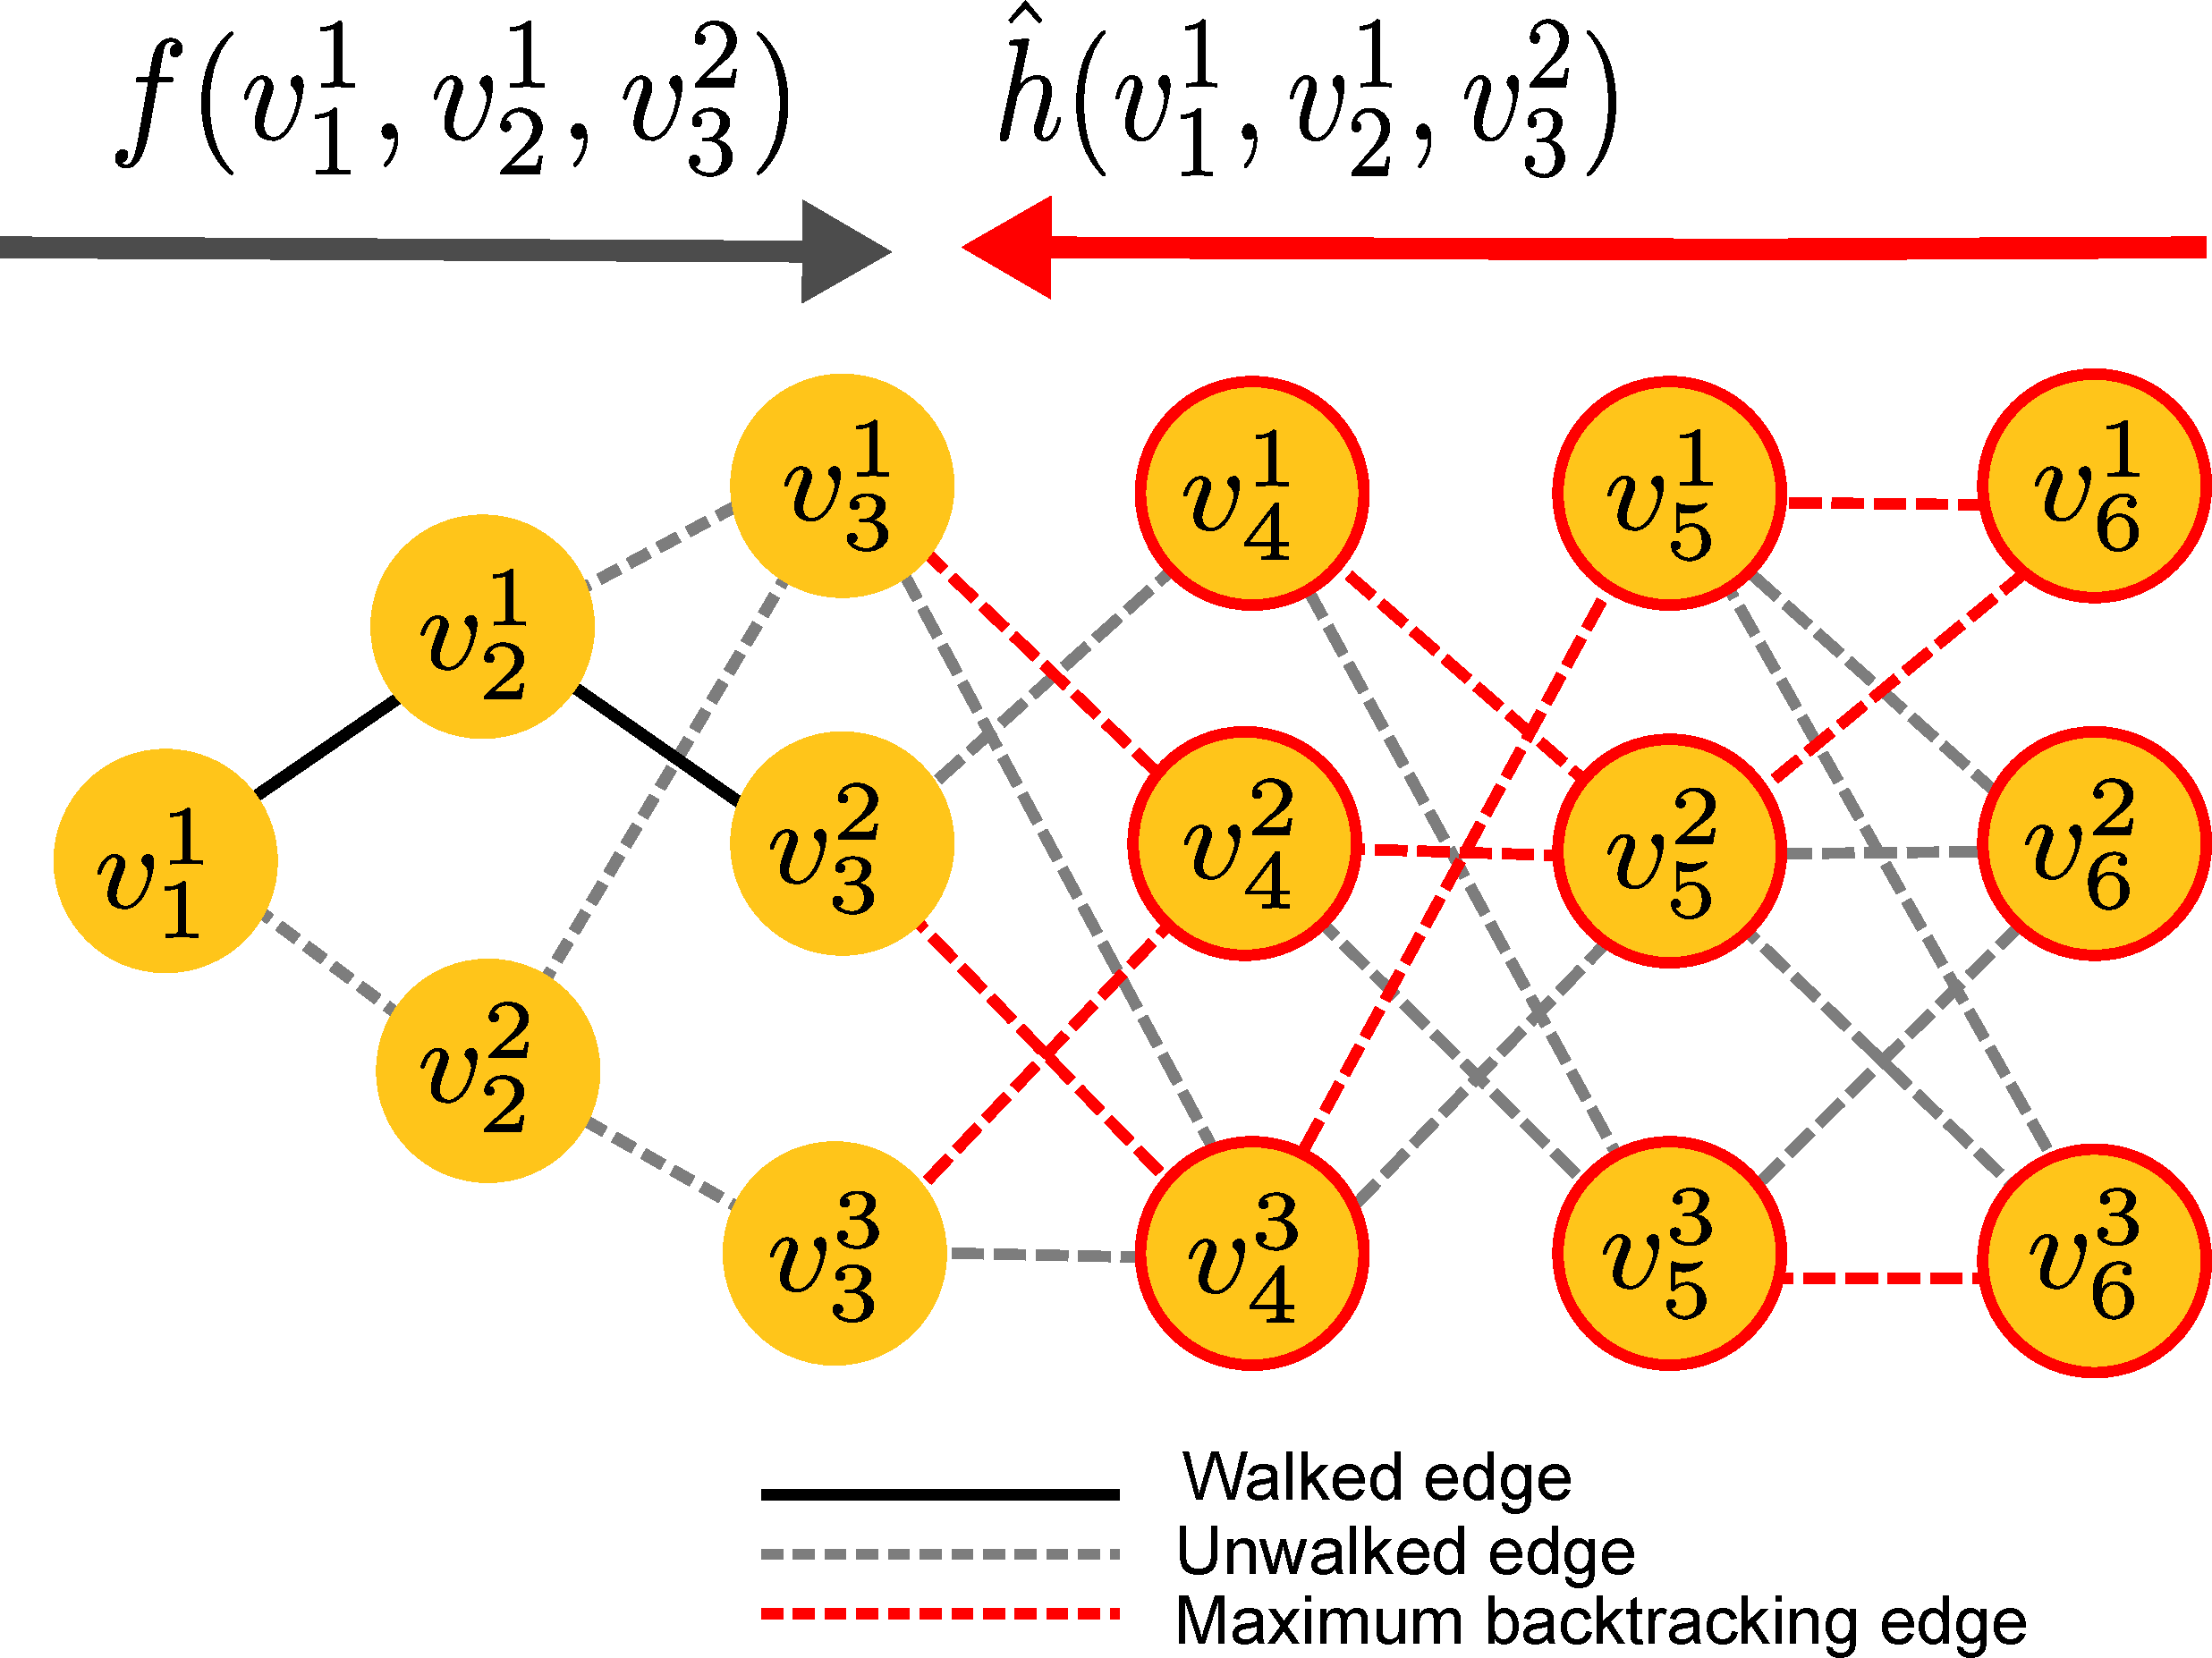
\includegraphics[width=0.5\linewidth]{./images/backtracking.pdf}
\caption{Backtracking process.}
\label{fig:backtracking}
\end{figure}

When we have $ \{ v_{1} , \cdots , v_{t'} \} $ visited, Algorithm \ref{alg:Backtrack} gives an estimated maximum future reward $ \hat{h}( v_{1} , \cdots , v_{t'} ) $. 
 
\begin{algorithm}
\caption{ $ \mathbf{BT}( \{ v_{1} , \cdots , v_{t'} \}, G ) $ - Backtracking }
\label{alg:Backtrack}
\begin{algorithmic}[1]
\REQUIRE
a sub-path $ \{ v_{1} , \cdots , v_{t'} \} $, and multi-partite graph $ G = ( V, E, T ) $
\ENSURE $ \hat{h}( v_{1} , \cdots , v_{t'} ) $ \\
\FOR{ $ t=T:-1:t'+1 $ }
\FOR{ $ v_{t} \in V(t) $}
\IF {$ t == T $}
\STATE $ \hat{u}(v_{T} \mid v_{1} , \cdots , v_{t'} ) = f(v_{T} \mid v_{1} , \cdots , v_{t'} ) $
\ELSE
\STATE $ \hat{h}( v_{1} , \cdots , v_{t'},  v_{t} ) = \max_{ { x_{t+1} \in V(t+1) } \land { (v_{t}, x_{t+1}) \in E } } \hat{u}(x_{t+1} \mid v_{1} , \cdots , v_{t'} ) $
\STATE $ \hat{u}(v_{t} \mid v_{1} , \cdots , v_{t'} ) = f(v_{t} \mid v_{1} , \cdots , v_{t'} ) + \hat{h}( v_{1} , \cdots , v_{t'} , v_{t}) $
\ENDIF
\ENDFOR
\ENDFOR
\STATE  $ \hat{h}( v_{1} , \cdots , v_{t'} ) = \max_{ {x_{t'+1} \in V(t'+1)} \land {(v_{t'}, x_{t'+1}) \in E} } \hat{u}(x_{t'+1} \mid v_{1} , \cdots , v_{t'} ) $
\RETURN $ \hat{h}( v_{1} , \cdots , v_{t'} )  $
\end{algorithmic}
\end{algorithm}
%Backtrack process provides all the possible future rewards of next step $ \hat{R}^{max}_{future}(x_{path(v).length+1} \mid path(v) ) $. Selecting the maximum, we can used this as the estimation on future reward of node $ v $, $ est_{max}(R^{max}_{future}(v)) $.

Algorithm \ref{alg:Backtrack} estimates the maximum total rewards of the vertices in a backward manner, which starts from time partition $ V(T) $ back to $ V(t'+1) $.
For each vertex $ v(t) $, the estimated maximum total reward $ \hat{u}(x_{t'+1} \mid v_{1} , \cdots , v_{t'} ) $ is a sum of the estimated instant reward and the estimated future reward.
The estimated instant reward is calculated by $ f(v_{t} \mid v_{1} , \cdots , v_{t'} ) $ .
The estimated future reward $ \hat{h}( v_{1} , \cdots , v_{t'} , v_{t}) $ is calculated by the following steps.
\begin{enumerate}
\item Find the vertex that has the biggest value of the estimated maximum total reward from the vertices in partition $ V(t+1) $ that are connected with $ v(t) $;
\item Take its estimated maximum total reward as the maximum future reward of $ v(t) $.
\end{enumerate}

We notice that there is an important property of the ``Backtracking'' defined in Algorithm \ref{alg:Backtrack}, which gives Lemma \ref{lem:underestimate}.

\begin{lem}
\label{lem:underestimate}
``Backtracking" in Algorithm \ref{alg:Backtrack} will never underestimate the maximum future reward, which means 
\begin{equation}
\label{eq:overestimate}
\hat{h}( v_{1} , \cdots , v_{t'} ) \geq h( v_{1} , \cdots , v_{t'} ).
\end{equation}
\begin{proof}

%By property \ref{prop:path}, we know that $ path(n_{t'}) $ defines a set of vertices in a sub-path $ \{ v_{1}, v_{2} , \cdots , v_{t'} \} $.
%Thus we need to look at maximum future reward $ h() $ and estimated maximum future reward $ \hat{h}() $ after $ \{ v_{1}, v_{2} , \cdots , v_{t'} \} $ visited. 

As defined in line 7 of Algorithm \ref{alg:Backtrack}, we can have
\begin{equation}
\label{eq:hatp_def}
\hat{u}( x_{t} \mid v_{1} , \cdots , v_{t'} ) = g(x_{t} \mid v_{1} , \cdots , v_{t'} ) + \hat{h}(v_{1} , \cdots , v_{t'}, x_{t} ).
\end{equation}
Similarly, as defined in line 6 of Algorithm \ref{alg:Backtrack}, we can have
\begin{equation}
\label{eq:hath2hatp}
\hat{h}( v_{1} , \cdots , v_{t'} ) = \max_{x_{t'+1} \in V(t'+1) \land (v_{t'}, x_{t'+1}) \in E} \hat{u}(x_{t'+1} \mid v_{1} , \cdots , v_{t'} ).
\end{equation}

By replacing the $ \hat{h}( v_{1} , \cdots , v_{t'} ) $ in equation \eqref{eq:overestimate} with equation \eqref{eq:hath2hatp} and replacing the $ h( v_{1} , \cdots , v_{t'} ) $ in equation \eqref{eq:overestimate} with equation \eqref{eq:h2p}, we can have
\begin{equation}
\label{eq:inductEnd}
\begin{aligned}
\max_{x_{t'+1} \in V(t+1) \land (v_{t'}, x_{t'+1}) \in E } \hat{u}(x_{t'+1} \mid v_{1} , \cdots , v_{t'} ) \geq \max_{x_{t'+1} \in V(t+1) \land (v_{t'}, x_{t'+1}) \in E } u(x_{t'+1} \mid v_{1} , \cdots , v_{t'} ).
\end{aligned}
\end{equation}

We prove equation \eqref{eq:overestimate} by using equation \eqref{eq:inductEnd} as an equivalence to prove.

By Property \ref{prop:u2gh_2}, we can express the maximum total reward in a form that approximates the steps in Algorithm \ref{alg:Backtrack} to facilitate the comparison.
We have, for any given time $ t > t' $,
\begin{equation}
\label{eq:def_g_2}
u( x_{t} \mid v_{1} , \cdots , v_{t'} ) = f( x_{t} \mid \tilde{x}_{t+1}, \cdots \tilde{x}_{T}, v_{1} , \cdots , v_{t'} ) +  \max_{x_{t+1} \in V(t+1) \land ( x_{t}, x_{t+1} ) \in E } u( x_{t+1} \mid v_{1} , \cdots , v_{t'} ).
\end{equation}

In estimating the total reward using Algorithm \ref{alg:Backtrack}, $ \{ \tilde{x}_{t+1}, \cdots , \tilde{x}_{T} \} $ is not predicted to apply into calculating instant reward of $ x_{t} $.
We have estimated maximum total reward$ \hat{u}(x_{t} \mid v_{1} , \cdots , v_{t'} ) $ as 
\begin{equation}
\label{eq:defHatG}
\begin{aligned}
\hat{u}( x_{t} \mid v_{1} , \cdots , v_{t'} ) = f( x_{t} \mid v_{1} , \cdots , v_{t'} ) + \max_{ x_{t+1} \in V(t+1) \land ( x_{t}, x_{t+1} ) \in E } \hat{u}( x_{t+1} \mid v_{1} , \cdots , v_{t'} ).
\end{aligned}
\end{equation}

Like the procedure of backtracking, we import an proof by induction from $ T $ back to $ t' + 1 $.

\textbf{Initial}

At time $ T $, we have
\begin{equation}
\label{eq:eqT1}
\begin{aligned}
u( x_{T} \mid  v_{1} , \cdots , v_{t'} ) = f( x_{T} \mid v_{1} , \cdots , v_{t'} ),
\end{aligned}
\end{equation}
and
\begin{equation}
\label{eq:eqT2}
\begin{aligned}
\hat{u}( x_{T} \mid v_{1} , \cdots , v_{t'} ) = f( x_{T} \mid v_{1} , \cdots , v_{t'} ).
\end{aligned}
\end{equation}

Combining equations \eqref{eq:eqT1} and \eqref{eq:eqT2}, we have
\begin{equation}
\label{eq:inductionInit}
\begin{aligned}
\forall x_{T} \in V(T), \hat{u}( x_{T} \mid v_{1} , \cdots , v_{t'} ) = u( x_{T} \mid v_{1} , \cdots , v_{t'} ).
\end{aligned}
\end{equation}

\textbf{Induction}

At any time $ t > t' $, assume that
\begin{equation}
\label{eq:inductionAssumption}
\begin{aligned}
\forall x_{t+1} \in V(t+1), \hat{u}(x_{t+1} \mid v_{1} , \cdots , v_{t'} ) \geq u(x_{t+1} \mid v_{1} , \cdots , v_{t'} ).
\end{aligned}
\end{equation}

Looking at the difference at time step $ t $ with  $ \hat{u}(\cdot) $ and $ u(\cdot) $ by equations \eqref{eq:def_g_2} and \eqref{eq:defHatG}, for any $ x_{t} $ we have

\begin{equation}
\label{eq:extendDifference}
\begin{aligned}
& \hat{u}( x_{t} \mid v_{1} , \cdots , v_{t'} ) - u(x_{t} \mid v_{1} , \cdots , v_{t'} ) \\
& = \left[( f( x_{t} \mid v_{1} , \cdots , v_{t'} ) + \max_{x_{t+1} \in V(t+1) \land (x_{t}, x_{t+1}) \in E } \hat{u}( x_{t+1} \mid v_{1} , \cdots , v_{t'} ) \right]  \\
& - \left[  f( x_{t} \mid v_{1} , \cdots , v_{t'}, \tilde{x}_{t+1}, \cdots \tilde{x}_{T} ) +  \max_{x_{t+1} \in V(t+1) \land ( x_{t}, x_{t+1} ) \in E } u( x_{t+1} \mid v_{1} , \cdots , v_{t'} ) \right]  \\
& = \left[ f(x_{t} \mid v_{1} , \cdots , v_{t'} ) - f(x_{t} \mid v_{1} , \cdots , v_{t'}, \tilde{x}_{t+1}, \cdots \tilde{x}_{T} ) \right] \\
& + \left[ \max_{ x_{t+1} \in V(t+1) \land ( x_{t}, x_{t+1} ) \in E } \hat{u}( x_{t+1} \mid v_{1} , \cdots , v_{t'} ) - \max_{x_{t+1} \in V(t+1) \land ( x_{t}, x_{t+1} ) \in E } u( x_{t+1} \mid v_{1} , \cdots , v_{t'} ) \right] .
\end{aligned}
\end{equation}

We can see that if 
\begin{equation}
\label{eq:inductionGEQ1}
f( x_{t} \mid v_{1} , \cdots , v_{t'} ) - f(x_{t} \mid v_{1} , \cdots , v_{t'}, \tilde{x}_{t+1}, \cdots \tilde{x}_{T} ) \geq 0,
\end{equation}
and
\begin{equation}
\label{eq:max_delta}
\max_{ x_{t+1} \in V(t+1) \land ( x_{t}, x_{t+1} ) \in E } \hat{u}( x_{t+1} \mid v_{1} , \cdots , v_{t'} ) - \max_{ x_{t+1} \in V(t+1) \land ( x_{t}, x_{t+1} ) \in E } u( x_{t+1} \mid v_{1} , \cdots , v_{t'} ) \geq 0.
\end{equation}
are both true, we can have
\begin{equation}
\label{eq:extendDifference_geq_0}
\hat{u}( x_{t} \mid v_{1} , \cdots , v_{t'} ) - u( x_{t} \mid v_{1} , \cdots , v_{t'} ) \geq 0
\end{equation}
proved. Thus we will prove equation \eqref{eq:inductionGEQ1} and equation \eqref{eq:max_delta} respectively.

By Lemma \ref{lem:submod}, we can prove equation \eqref{eq:inductionGEQ1} directly.

Then we are going to prove equation \eqref{eq:max_delta} is also true.

Let 
\begin{equation}
\label{eq:arg_x_a}
x^{a}_{t+1} = \arg \max_{ x_{t+1} \in V(t+1) \land ( x_{t}, x_{t+1} ) \in E} \hat{u}( x_{t+1} \mid v_{t'} , \cdots , v_{1} )
\end{equation}
and 
\begin{equation}
\label{eq:arg_x_b}
x^{b}_{t+1} = \arg \max_{ x_{t+1} \in V(t+1) \land ( x_{t}, x_{t+1}) \in E } u( x_{t+1} \mid v_{1} , \cdots , v_{t'} ). 
\end{equation}

$ x^{a}_{t+1} $ and $ x^{b}_{t+1} $ can be either same or different. Both two belong to same set satisfying $ x_{t+1} \in V(t+1) \land (x_{t}, x_{t+1}) \in E $.

Since $ x^{a}_{t+1} $ is the answer to $ \arg \max \hat{u}(\cdot) $, we have
\begin{equation}
\label{eq:bigger1}
\begin{aligned}
\hat{u}( x^{a}_{t+1} \mid v_{1} , \cdots , v_{t'} ) \geq \hat{u}( x^{b}_{t+1} \mid v_{1} , \cdots , v_{t'} ).
\end{aligned}
\end{equation}


By equation \eqref{eq:inductionAssumption},
\begin{equation}
\label{eq:bigger2}
\begin{aligned}
\hat{u}( x^{b}_{t+1} \mid v_{1} , \cdots , v_{t'} ) \geq u( x^{b}_{t+1} \mid v_{1} , \cdots , v_{t'} ).
\end{aligned}
\end{equation}

Combining equations \eqref{eq:bigger1} and \eqref{eq:bigger2} using transitivity, we have 
\begin{equation}
\label{eq:bigger_trans}
 \hat{u}( x^{a}_{t+1} \mid v_{1} , \cdots , v_{t'} ) \geq  u ( x^{b}_{t+1} \mid v_{1} , \cdots , v_{t'} ).
\end{equation}

By the definitions in equations \eqref{eq:arg_x_a} and \eqref{eq:arg_x_b}, equation \eqref{eq:bigger_trans} is equivalent to equation \eqref{eq:max_delta}. Thus equation \eqref{eq:max_delta} is true.

With equations \eqref{eq:inductionGEQ1} and \eqref{eq:max_delta}, we have
\begin{equation}
\label{eq:inductConclusion}
\forall x_{t} \in V(t), \hat{u}( x_{t} \mid v_{1} , \cdots , v_{t'} ) \geq u( x_{t} \mid v_{1} , \cdots , v_{t'} ).
\end{equation}

Thus, we have
\begin{equation}
\label{eq:induction}
\begin{aligned}
\forall x_{t+1} \in V(t+1), \hat{u}( x_{t+1} \mid v_{1} , \cdots , v_{t'} ) \geq u( x_{t+1} \mid v_{1} , \cdots , v_{t'} )  \\
\Rightarrow  \forall x_{t} \in V(t), \hat{u}( x_{t} \mid v_{1} , \cdots , v_{t'} ) \geq u( x_{t} \mid v_{1} , \cdots , v_{t'} ).
\end{aligned}
\end{equation}

\textbf{Conclusion}

Using equations \eqref{eq:inductionInit} and \eqref{eq:induction}, we can apply induction from $ T $ to $ t'+1 $ to get
\begin{equation}
\label{eq:inductionResult}
\forall x_{t'+1} \in V(t'+1), \hat{u}( x_{t'+1} \mid v_{1} , \cdots , v_{t'} ) \geq u( x_{t'+1} \mid v_{1} , \cdots , v_{t'} ).
\end{equation}

Applying $ max(\cdot) $ operator on equation \eqref{eq:inductionResult} gets equation \eqref{eq:inductEnd}.
Equation \eqref{eq:inductEnd} has been proved, which means that equation \eqref{eq:overestimate} stands.
So we arrive to the conclusion that ``Backtracking" in Algorithm \ref{alg:Backtrack} will never underestimate the future reward.

\end{proof}
\end{lem}

\subsection{Tree Expanding Search}
\label{subsec:tree_expanding_search}

Recall that $ path(n_{t}) $ of a node $ n_{t} $ in the expanding tree $ G_{T} $ maps to a unique path in the multi-partite graph $ G $ in Property \ref{prop:path}.
We model the process of path search on the multi-partite graph $ G $ as a tree expanding process.
A backtracking process can generate estimated maximum future rewards for all the vertices in the unvisited partitions.
Since the backtracking process does not guarantee that there is no bias on the estimation, the first complete path created in the expanding tree might not be the optimal solution.
If the search does not stop at finding one complete solution, the expanding tree $ G_{T} $ can be used to track whether a vertex in a path on the multi-partite graph $ G $ has been explored and to store its estimated rewards.
Adding a node $ n^{i(j)}_{t} $ means that a sub-path $ path( n^{i(j)}_{t} ) $ has been explored on the multi-partite graph $ G $.
``Expanding'' a node includes adding the children of node $ n_{t} $ to our $ G_{T} $ data structure and storing the estimated rewards of a sub-path $ path(n_{t}) $ in node $ n_{t} $ by ``backtracking''.

Here we assign a state to each node $ n_{t} $ to facilitate the history tracking in the search process. 
There are three types of states:
\begin{description}
\item [New] a node has been created but not expanded;
\item [Expanded] a node that has all child nodes created;
\item [Frozen] a node that has been created but will not be expanded.
\end{description}

In order to have a better approximation to the true value of $ h() $, we will call Algorithm \ref{alg:Backtrack} to estimate the maximum future reward for the newly added nodes
\footnote{A proof on that estimating maximum future reward with newly added vertex provides a better approximation to the $ h() $ is given in Appendix \ref{app:better_approximation} }. 
Integrating ``recursive backtracking" into a ``node expanding'' process, we propose Algorithm \ref{alg:RecursiveBacktrack}.
Since each expanding node indicates a sub-path from the root node, Algorithm \ref{alg:RecursiveBacktrack} can start from any expanding node $ n_{t'} $ and concatenate the sub-path $ path(n_{t'}) $ to generate a complete path solution.

\begin{algorithm}
\caption{ $ \mathbf{NERB}( n_{t'}, G, G_{T} ) $ - Node Expanding with Recursive Backtracking }
\label{alg:RecursiveBacktrack}
\begin{algorithmic}[1]
\REQUIRE 
Expanding Node $ n_{t'} $, Multi-partite graph $ G = (V, E, T) $, Expanding tree $ G_{T} = (N, L, T) $
\ENSURE $ solution $ of a complete path
\STATE $ solution = path(n_{t'}) $ 
\FOR{ $ t=t':1:T-1 $ }
\STATE  Expand node $ n_{t'} $ to get $ child(n_{t'}) $
\STATE  $ n_{t'}.state = \mbox{\emph{Expanded}} $
\STATE  $ child(n_{t'}) = \{ n_{t'+1} \mid v(n_{t'+1}) \in V(t'+1) \land (v(n_{t'}), v(n_{t'+1})) \in E  \} $
\FOR{ $ n_{t'+1} $ in $ child(n_{t'}) $ }
\STATE  calculate $ f(path(n_{t'+1})) $
\STATE  $ \hat{h}(path(n_{t'+1})) = \mathbf{BT}( path(n_{t'+1}) , G ) $
\ENDFOR
\STATE  $ \hat{n}_{t'+1} = \arg \max_{n_{t'+1} \in child(n_{t'})} \hat{h}(path(n_{t'+1})) $
\STATE  $ solution = solution \bigcup \{ \hat{n}_{t'+1} \} $
\ENDFOR 
\RETURN $ solution $
\end{algorithmic}
\end{algorithm}

In Algorithm \ref{alg:RecursiveBacktrack}, $ child() $ is defined for a set of the children nodes of an expanding node $ n_{t'} $, which is generated from a set of all the vertices in $ V(t'+1) $ that are connected with $ v(n_{t'}) $.
We are able to get a solution of a complete path using Algorithm \ref{alg:RecursiveBacktrack} by recursively estimate $ \hat{h}(path(n_{t})) $ at each time step $ t $.
Each single run of Algorithm \ref{alg:RecursiveBacktrack} reaches a terminal node in the expanding tree.
By the heuristic from backtracking estimation, a complete path can be optimal or near optimal.
The optimality depends on how the correctness on estimating maximum future reward influence the optimal solution search.

\subsection{Anytime Algorithm Framework}
\label{subsec:anytime_algorithm_framework}

The tree expanding search naturally implies an anytime algorithm framework. 
In this section, we formalize the tree expanding search as an anytime algorithm framework.
It means that we have a solution from the first single call of Algorithm \ref{alg:RecursiveBacktrack} and continues to search for a potential better solution. 

In avoid of an exhaustive search, we propose a node freeze process to prune those nodes that are impossible to reach an optimal terminal node. ``Freezing" a node means never exploring the child nodes of a node, which works in a similar way with pruning in search. 

\begin{figure}
\centering
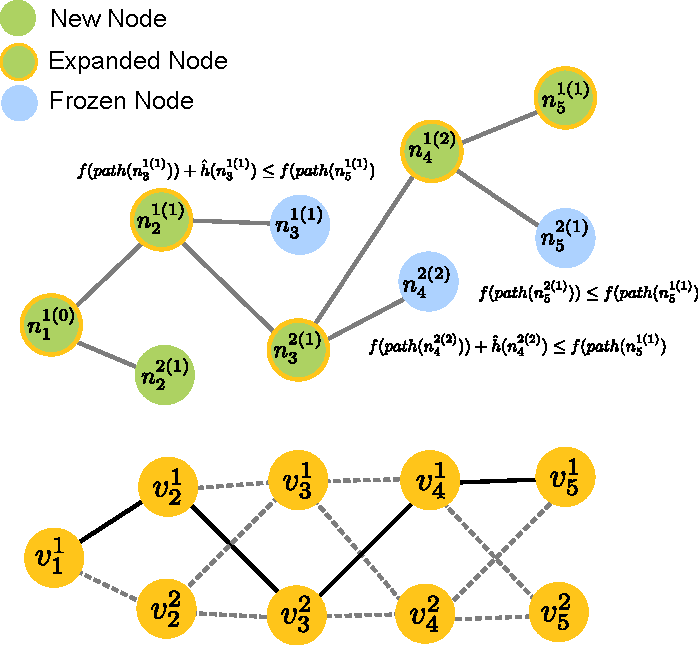
\includegraphics[width=0.7\linewidth]{./images/freeze_process.pdf}
\caption{Node freeze process.}
\label{fig:freeze_process}
\end{figure}

By Lemma \ref{lem:underestimate}, if the estimated maximum total reward of a node in an expanding tree is smaller than the total reward of current best path, it is impossible that this node locates in a complete path that has bigger total reward.
We are not interested with any descendant nodes of this node, thus freeze this node.
A node is frozen means that the sub-tree structure from this node will never be explored.
The node freeze process is used to update the states of the nodes in an expanding tree, which is given in Algorithm \ref{alg:FreezeNode}.

\begin{algorithm}
\caption{Node Freeze}
\label{alg:FreezeNode}
\begin{algorithmic}[1]
\REQUIRE 
an expanding tree $ G_{T} = (N, L, T) $, the current best terminal node $ \hat{n}^{*}_{T} $
\STATE $ \theta = f(path(\hat{n}^{*}_{T})) $
\FOR{$ n_{t} \in N $ \AND $ n_{t}.state == \mbox{\emph{New}} $}
\IF{ $ \hat{h}(path(n_{t})) + f(path(n_{t})) \leq \theta $ }
\STATE $ n_{t}.state = \mbox{\emph{Frozen}} $
\ENDIF
\ENDFOR
\end{algorithmic}
\end{algorithm}

After all the sub-procedures given, we can form the ``anytime algorithm framework''.
An expanding tree starts from a structure with only a root node - start position.
When a node is initially created, the state of the node is \emph{New}.
Algorithm \ref{alg:Backtrack} expands a node by creating all its child nodes and changes the state of the node to \emph{Expanded}.
The estimating maximum total rewards of all child nodes will also be calculated and stored.
After first run of Algorithm \ref{alg:RecursiveBacktrack}, an optimal or near-optimal complete path is obtained.
When a new complete path has been found, a freeze process defined in \ref{alg:FreezeNode} will be executed by checking estimated total rewards stored in each nodes in the state of \emph{New}.
If there is enough calculating time budget that allows a next run of search, the framework will find a node $ n_{t} $ that has the largest estimated total reward $ \hat{h}(path(n_{t})) + f(path(n_{t})) $.
Starting from this node, a next call to Algorithm \ref{alg:RecursiveBacktrack} will find another complete path.
This anytime algorithm framework is stopped by some stopping criteria or that there is no node of state $ New $ left.
The process is given in Algorithm \ref{alg:Anytime}.

\begin{algorithm}
\caption{Anytime Algorithm Framework}
\label{alg:Anytime}
\begin{algorithmic}[1]
\REQUIRE 
Expanding Tree $ G_{T} = (N, L, T) $, and multi-partite graph $ G = (V, E, T) $;
\STATE Initial expanding tree $ G_{t}(N, L, T) $ with $ v_{1} $ as root node
\STATE $ maxPath = NULL $, $ newPath = NULL $
\STATE $ n' = G_{T}.root $
\WHILE { $ n' != NULL $ }
\STATE $ newPath = \mathbf{NERB}( n', G, G_{T} ) $
\IF {$ (f(newPath) > f(maxPath))  $}
\STATE $ maxPath = newPath $
\STATE post $ maxPath $
\ENDIF
\STATE Call ``Node Freeze" of Algorithm \ref{alg:FreezeNode}
\STATE $ n' = \arg \max_{ \{n \mid n \in N \land n.state == \mbox{\emph{New}} \} } \hat{h}(path(n)) $
\ENDWHILE 
\end{algorithmic}
\end{algorithm}

We propose that theorem \ref{thm:optimal} stands on the anytime algorithm framework in Algorithm \ref{alg:Anytime}.

\begin{thm} 
\label{thm:optimal}
The anytime algorithm framework in Algorithm \ref{alg:Anytime} can always find an optimal solution given enough run time.
\begin{proof}

Finding the optimal solution equals to reaching a terminal node in the optimal path of the expanding tree.
Since Algorithm \ref{alg:Anytime} keeps expanding new nodes till that there is no node in state \emph{New}, as long as any node in the optimal path will never be frozen, the search will reach the optimal terminal node.

Assume that one of the node $ n^{*}_{t} $ in the optimal path can be frozen. It means that 
\begin{equation}
\label{eq:contra_assumption}
\hat{h}(path(n^{*}_{t})) + f(path(n^{*}_{t})) \leq f(path(n'_{T})),
\end{equation}
in which $ n'_{T} $ is another terminal node but not optimal terminal node.
As a result, when $ n'_{T} $ has been reached, it will freeze node $ n^{*}_{t} $. 

However, as node $ n^{*}_{t} $ is in a path to an optimal terminal node, $ f(path(n^{*}_{t})) + h(path(n^{*}_{t})) > f(path(n'_{T})) $.
Also we have $ f(path(n^{*}_{t})) + \hat{h}(path(n^{*}_{t})) \geq f(path(n^{*}_{t})) + h(path(n^{*}_{t})) $ by Lemma \ref{lem:underestimate}.
Thus we have $ f(path(n^{*}_{t})) + \hat{h}(path(n^{*}_{t}) > f(path(n'_{T})) $. It contradict with equation \eqref{eq:contra_assumption}.

Therefore, an node in a path to an optimal terminal node will never be frozen by any non-optimal terminal node.
It guarantees that an optimal terminal node will always be reached given enough run times.
It means that the anytime algorithm framework in Algorithm \ref{alg:Anytime} can always find an optimal solution.

\end{proof}
\end{thm}